\documentclass[uplatex,a4paper,12pt]{jsarticle}
% \documentclass[uplatex,a4paper,12pt,draft]{jsarticle}

%% フォント
%\usepackage{newtxtext,newtxmath}
%% 図、文字色
\usepackage[dvipdfmx]{graphicx,xcolor}
%% ハイパーリンク
\usepackage[dvipdfmx]{hyperref}
%% しおりの日本語
\usepackage{pxjahyper}
%% しおりに節番号を含める、リンクの枠を出力しない
\hypersetup{
  bookmarksnumbered=true,
  hidelinks=true,
  colorlinks=false,
}
%% 特殊記号
\usepackage{textcomp}
%% URL
\usepackage{url}
%% 表
%\usepackage{multirow}
%% 参照漏れチェック
%\usepackage{refcheck}

\usepackage{subcaption}

% 図と表の表記
\renewcommand{\figurename}{Fig.}
\renewcommand{\tablename}{Table.}
\newcommand{\figref}[1]{\figurename~\ref{#1}}
\newcommand{\tabref}[1]{\tablename~\ref{#1}}

\usepackage[top=30truemm,bottom=30truemm,left=30truemm,right=30truemm]{geometry}

\begin{document}

% 表紙
\begin{picture}(420,520)(-20,20)
%契約番号(必須)
\put(330,470){\makebox(50,5)[l]{\normalsize{2023情財第 XXX 号}}} %「XXX」はプロジェクトごとの番号に置き換える
%事業名(必須)
\put(140,350){\makebox(100,15)[c]{\LARGE{2023年度未踏IT人材発掘・育成事業}}}
%プロジェクト名
\put(140,320){\makebox(100,15)[c]{\LARGE{ぬいぐるみ専用の組み込みAIモジュールの開発}}}
% \put(140,290){\makebox(100,15)[c]{\LARGE{契約名2行目(必要なら)}}}
\put(140,290){\makebox(100,15)[c]{\LARGE{成果報告書}}} %2行目がなければ\put(140,290)
%クリエータ名1(必須、人数に応じて\putの位置を調整)
\put(140,140){\makebox(100,10)[c]{\Large{クリエータ:小山 高}}}
%クリエータ名2(必須、人数に応じて\putの位置を調整)
% \put(140,110){\makebox(100,10)[c]{\Large{      姓 名}}}
% 担当PM名(クリエータ2がいなければ\put(140,100)
\put(140,100){\makebox(100,10)[c]{\Large{担当PM:稲見 昌彦}}}
%日付(必須、通常は契約最終日、クリエータ2がいなければ\put(140,60)
\put(140,60){\makebox(100,15)[c]{\Large{2024年3月8日}}}
\end{picture}
\thispagestyle{empty}
\clearpage

\tableofcontents
\thispagestyle{empty}
\clearpage

% 本文
\pagenumbering{arabic}
\setcounter{page}{1}

\section{要約}
本プロジェクトでは、様々な種類のぬいぐるみをロボット化するための、ぬいぐるみ専用の組み込みAIモジュールを提案・実装した。
ぬいぐるみロボットでは、人の好みに寄り添うために、多くの種類のぬいぐるみに対応する必要がある。
そこで、ぬいぐるみロボットを、機械的・電気的要素を含む共通の骨格とぬいぐるみを成す毛皮、ソフトウェアによる知能という三要素に分割して解決したのが本プロジェクトの特徴である。
本プロジェクトでは実際にぬいぐるみロボットを製作し、共通の内部骨格を用いたぬいぐるみ部分の換装の検証や、人とのインタラクションの検証を行った。

\section{背景及び目的}
本プロジェクトでは、現代を生きる若者の孤独に着目し、彼らの生活様式に即した癒やしの手段としてぬいぐるみロボットを提案する。


\subsection{学生の孤独とペットによる癒やし}
2020年に始まった新型コロナウイルスの流行によって大学ではオンライン授業が行われ、同時に学生同士のつながりが希薄になった。
特に一人暮らしの学生は話す相手が極端に減少するなど、生活面や精神面で大きな苦痛を強いられたものと考えられる。
実際に筆者の所属する大学も授業が対面形式からオンライン授業に移行し、1か月以上誰とも話す機会がなくコミュニケーションの不足に苦しんだ経験がある。
そして、コロナ禍が収まった後であっても、当時の大学内外の交流のきっかけが失われたことが尾を引き、現在も孤独に陥る学生が筆者を含め多く存在すると考えられる。

コミュニケーションは人が心身ともに健康に生活する上で欠かせないものであるが、その相手は必ずしも人とは限らない。
例えば、コロナ禍の時期には、癒やしや巣ごもり需要としてペットの飼育が一時的な流行となった~\cite{web_pet}。
動物との触れ合いは人の心に安らぎを与えると言われている。
しかし、一人暮らしの大学生がペットを飼うことは容易ではない。
例として、ペットとして一般的な犬を飼育する場合は毎日散歩などの世話が必要となり、犬の生涯にかけて250万円ほどの経費が掛かるとされている~\cite{web_petfood}。

このように、ペットは癒やしを得るには効果的な一方で、その維持管理に必要なコストが高いという問題点がある。


\subsection{愛玩用ロボット}
ペットの維持管理の手間を減らしたいニーズに応えてか、手軽に癒やしを得られる愛玩用ロボットがいくつか販売されている。

例えば、犬のような外見をした家庭用ロボットaibo~\cite{web_aibo}、アザラシのような介護現場でも用いられるロボットのパロ~\cite{web_paro}、車輪で駆動する家庭用ロボットLOVOT~\cite{web_lovot}などが存在する(\figref{fig:previous_robots_expensive})。
これらはセンサを多用することでユーザの振る舞いに呼応する機能が埋め込まれており、30万円~50万円で販売されている。

一方で、手のひらサイズのロボットMoflin~\cite{web_moflin}や可動式の尻尾付きのQoobo~\cite{web_qoobo}、ぬいぐるみに縫い付けて使用するボタン型スピーカーpechat~\cite{web_pechat}(※2024年2月で販売終了)といった5万円以下の比較的安価な愛玩用ロボットも存在する(\figref{fig:previous_robots_inexpensive})。
これらは機能や用途を限定しつつもユーザに安らぎや楽しみをもたらすことを目指している。

しかし、これらの愛玩用ロボットは未だ市場に広くは出回っておらず、人々認知度も低い。
さらに、工業製品であるがゆえに同型のロボットは多少の色違いこそあれ、基本的にはすべて同じ形である。
これでは、愛玩の対象として重要な、自分の目の前の相手がこの世にただ一人しかいないことから来る愛着、つまりオンリーワンの要素に乏しい。


\begin{figure}[htbp]
  \centering
  \begin{minipage}[c]{0.32\linewidth}
    \centering
    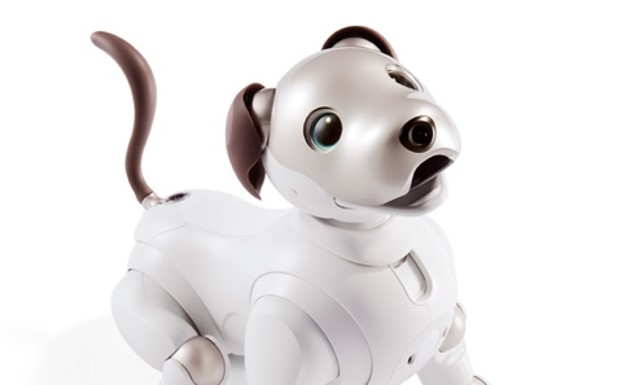
\includegraphics[keepaspectratio,width=4cm,clip]{images/previous_robots/aibo.jpg}
    \subcaption{aibo~\cite{web_aibo}}
    \label{fig:aibo}
  \end{minipage}
  \begin{minipage}[c]{0.32\linewidth}
    \centering
    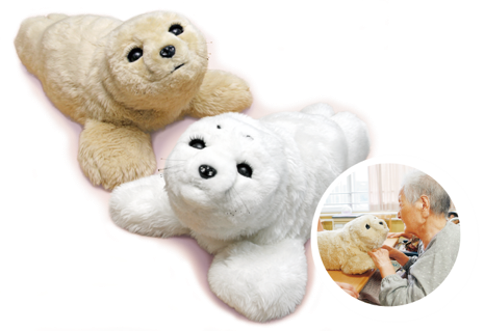
\includegraphics[keepaspectratio,width=4cm,clip]{images/previous_robots/paro.png}
    \subcaption{パロ~\cite{web_paro}}
    \label{fig:paro}
  \end{minipage}
  \begin{minipage}[c]{0.32\linewidth}
    \centering
    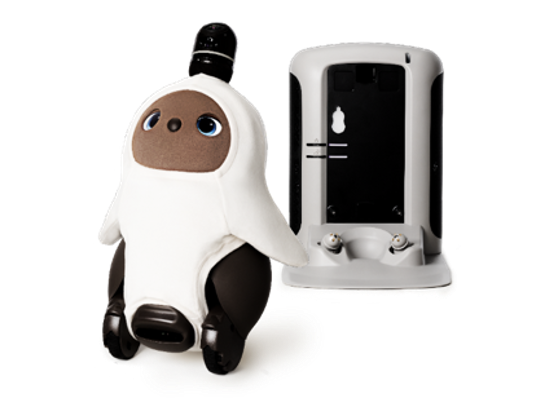
\includegraphics[keepaspectratio,width=4cm,clip]{images/previous_robots/lovot.png}
    \subcaption{LOVOT~\cite{web_lovot}}
    \label{fig:lovot}
  \end{minipage}
  \caption{愛玩用ロボットの例(高価格帯)}
  \label{fig:previous_robots_expensive}
\end{figure}

\begin{figure}[htbp]
  \centering
  \begin{minipage}[c]{0.32\linewidth}
    \centering
    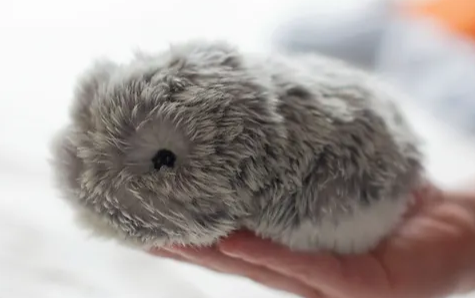
\includegraphics[keepaspectratio,width=4cm,clip]{images/previous_robots/moflin.png}
    \subcaption{Moflin~\cite{web_moflin}}
    \label{fig:moflin}
  \end{minipage}
  \begin{minipage}[c]{0.32\linewidth}
    \centering
    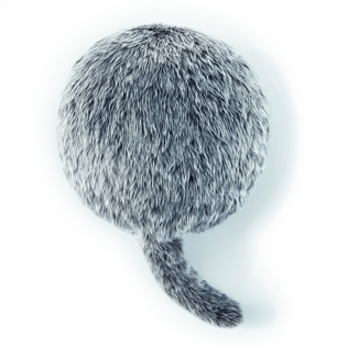
\includegraphics[keepaspectratio,width=4cm,clip]{images/previous_robots/qoobo.png}
    \subcaption{Qoobo~\cite{web_qoobo}}
    \label{fig:qoobo}
  \end{minipage}
  \begin{minipage}[c]{0.32\linewidth}
    \centering
    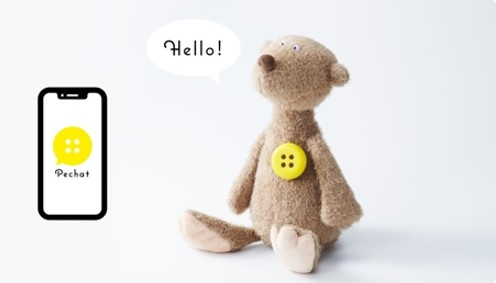
\includegraphics[keepaspectratio,width=4cm,clip]{images/previous_robots/pechat.jpg}
    \subcaption{pechat~\cite{web_pechat}}
    \label{fig:pechat}
  \end{minipage}
  \caption{愛玩用ロボットの例(低価格帯)}
  \label{fig:previous_robots_inexpensive}
\end{figure}


\subsection{ぬいぐるみの特徴}

そこで、人々に親しまれているぬいぐるみをロボットにすることを考える。
ぬいぐるみにはいくつかの特徴があるが、筆者の経験をもとにぬいぐるみの魅力を以下に述べる。

第一に、ぬいぐるみはその可愛らしい見た目ともふもふとした柔らかい触り心地から、落ち着きを与えてくれる。
幼い子どもがぬいぐるみとともに就寝するというのはよく見られる光景であろう。

次に、ぬいぐるみは自発的に動く存在ではなく、持ち主が触れ合いたいと考えたときだけ触れ合える。
これは、ぬいぐるみは持ち主の生活を縛らない、適度な距離感を持った愛玩対象であることを示す。
また、手入れの手間もほとんどかからないため、複数所持することは容易であり、使わない場合は長期間しまっておくことも可能である。

さらに、ぬいぐるみは人の心を投影する対象ともなりうる。
例えば図では女性が赤ちゃんにぬいぐるみを通して語りかけているが、これは女性の感情をぬいぐるみに代弁させているとも捉えられる。
つまり、ぬいぐるみとは愛玩対象であるとともに自身の代弁者ともなり、人とのコミュニケーションにおいて面と向かって伝えづらいこともぬいぐるみを通して語れるといった、コミュニケーションに彩りを持たせ、円滑に進める働きもある。

最後に、ぬいぐるみは実に多様な見た目のものが存在する。
例えば本物の動物であれば、その大きさなどの物理的制約から、実際に飼育できるものは犬や猫、小動物といったものに限られる。
一方で、ぬいぐるみは多くの種類が存在し、より個人の好みに寄り添う存在となっている。
例えば図ではアザラシやペンギン、ホッキョクグマなどを模したぬいぐるみが確認できるが、一つの店だけで50種類近くの品揃えがあることも珍しくない。
付け加えて重要なのが、これらのぬいぐるみはしばしば種々のイベントに合わせて贈られる文化が存在する点である。
子どもが誕生日に親からぬいぐるみを贈られたり、旅先の動物園や水族館、旅館等で土産に買ってもらったりすることは一般的な光景である(\figref{fig:zoo})。
そして、これらのぬいぐるみの多様性やそれにまつわる想い出は、目の前のぬいぐるみがオンリーワンの存在である印象を持ち主に与え、単なる布と綿からできた工業製品以上の愛着をもたらしうる。

\begin{figure}[htbp]
  \centering
  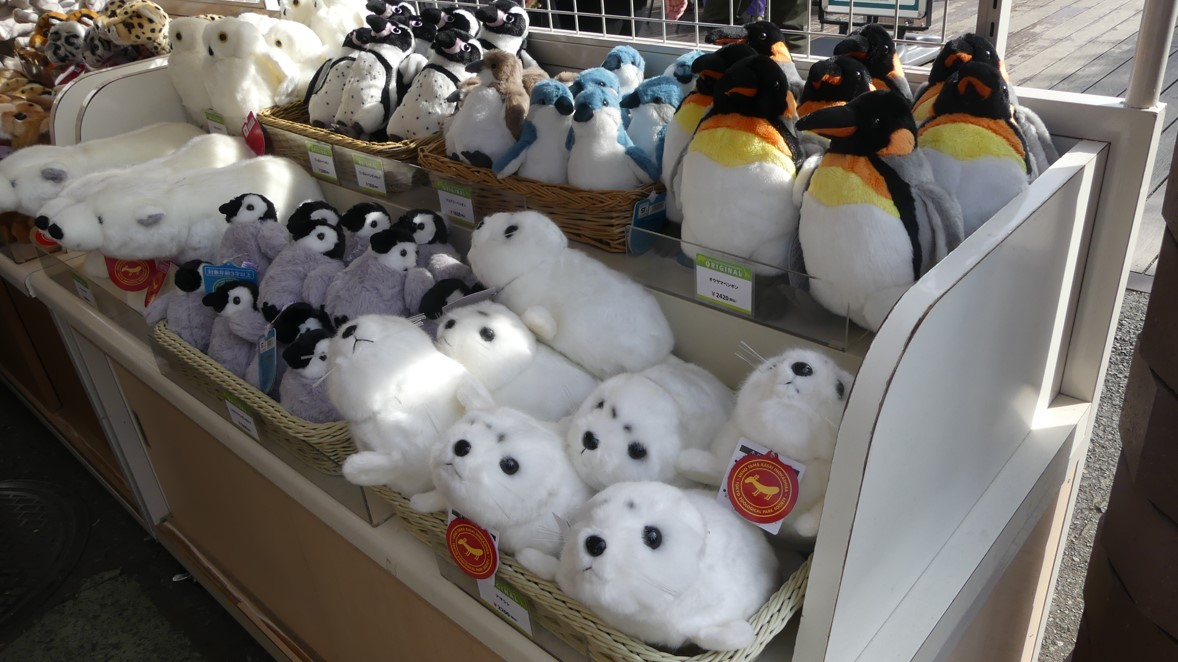
\includegraphics[width=8cm]{images/backgrounds/zoo.jpg}
  \caption{動物園でのぬいぐるみの販売風景}
  \label{fig:zoo}
\end{figure}

このように、ぬいぐるみには様々な魅力がある一方で、それらが逆に問題となることもある。
前述のとおり、ぬいぐるみは触れ合えいたいときだけ触れ合える存在であるが、裏を返せば持ち主の働きかけがない限り決して動かないことを意味し、愛玩対象としてはやや魅力に欠ける一面がある。

本プロジェクトでは、ぬいぐるみについて、その魅力を活かしつつも、さらなる愛着を抱ける対象に発展させることを目指した。
そこで、本プロジェクトでは複数の種類のぬいぐるみを効率的にロボット化できるモジュールを開発し、持ち主の好みに寄り添ったぬいぐるみが命を吹き込まれたかのように振る舞うシステムの構築を検討した。



\section{プロジェクト概要}
本プロジェクトではぬいぐるみ専用の組み込みAIモジュールを開発し、あらゆる種類のぬいぐるみにロボティクスを適用する。
そして、幅広いぬいぐるみに効率的に知能を埋め込むためのプラットフォームの構築を目指す。

本プロジェクトでは、ぬいぐるみのロボット化に特化した組み込みAIモジュールを開発し、ぬいぐるみの骨格の規格化を目指す。
そして、ぬいぐるみの毛皮と骨格の開発過程を分離することで、幅広いぬいぐるみに効率的に知能を埋め込むための土台を築き上げる。

\section{開発内容}
\subsection{ぬいぐるみロボットシステムMohuticsの構成}
本プロジェクトでは、ぬいぐるみロボットを大きく以下の三要素に分割する(\figref{fig:mohutics:concept})。
\begin{description}
  \item[MohuCore(もふこあ)] ロボットの機械的・電気的要素を含む共通化された骨格部分
  \item[MohuKawa(もふかわ)] ロボットの内部骨格MohuCoreを覆うぬいぐるみ(毛皮)部分
  \item[MohuAI(もふあい)] ロボットに書き込むソフトウェア(知能)部分
\end{description}

\begin{figure}[htbp]
  \centering
  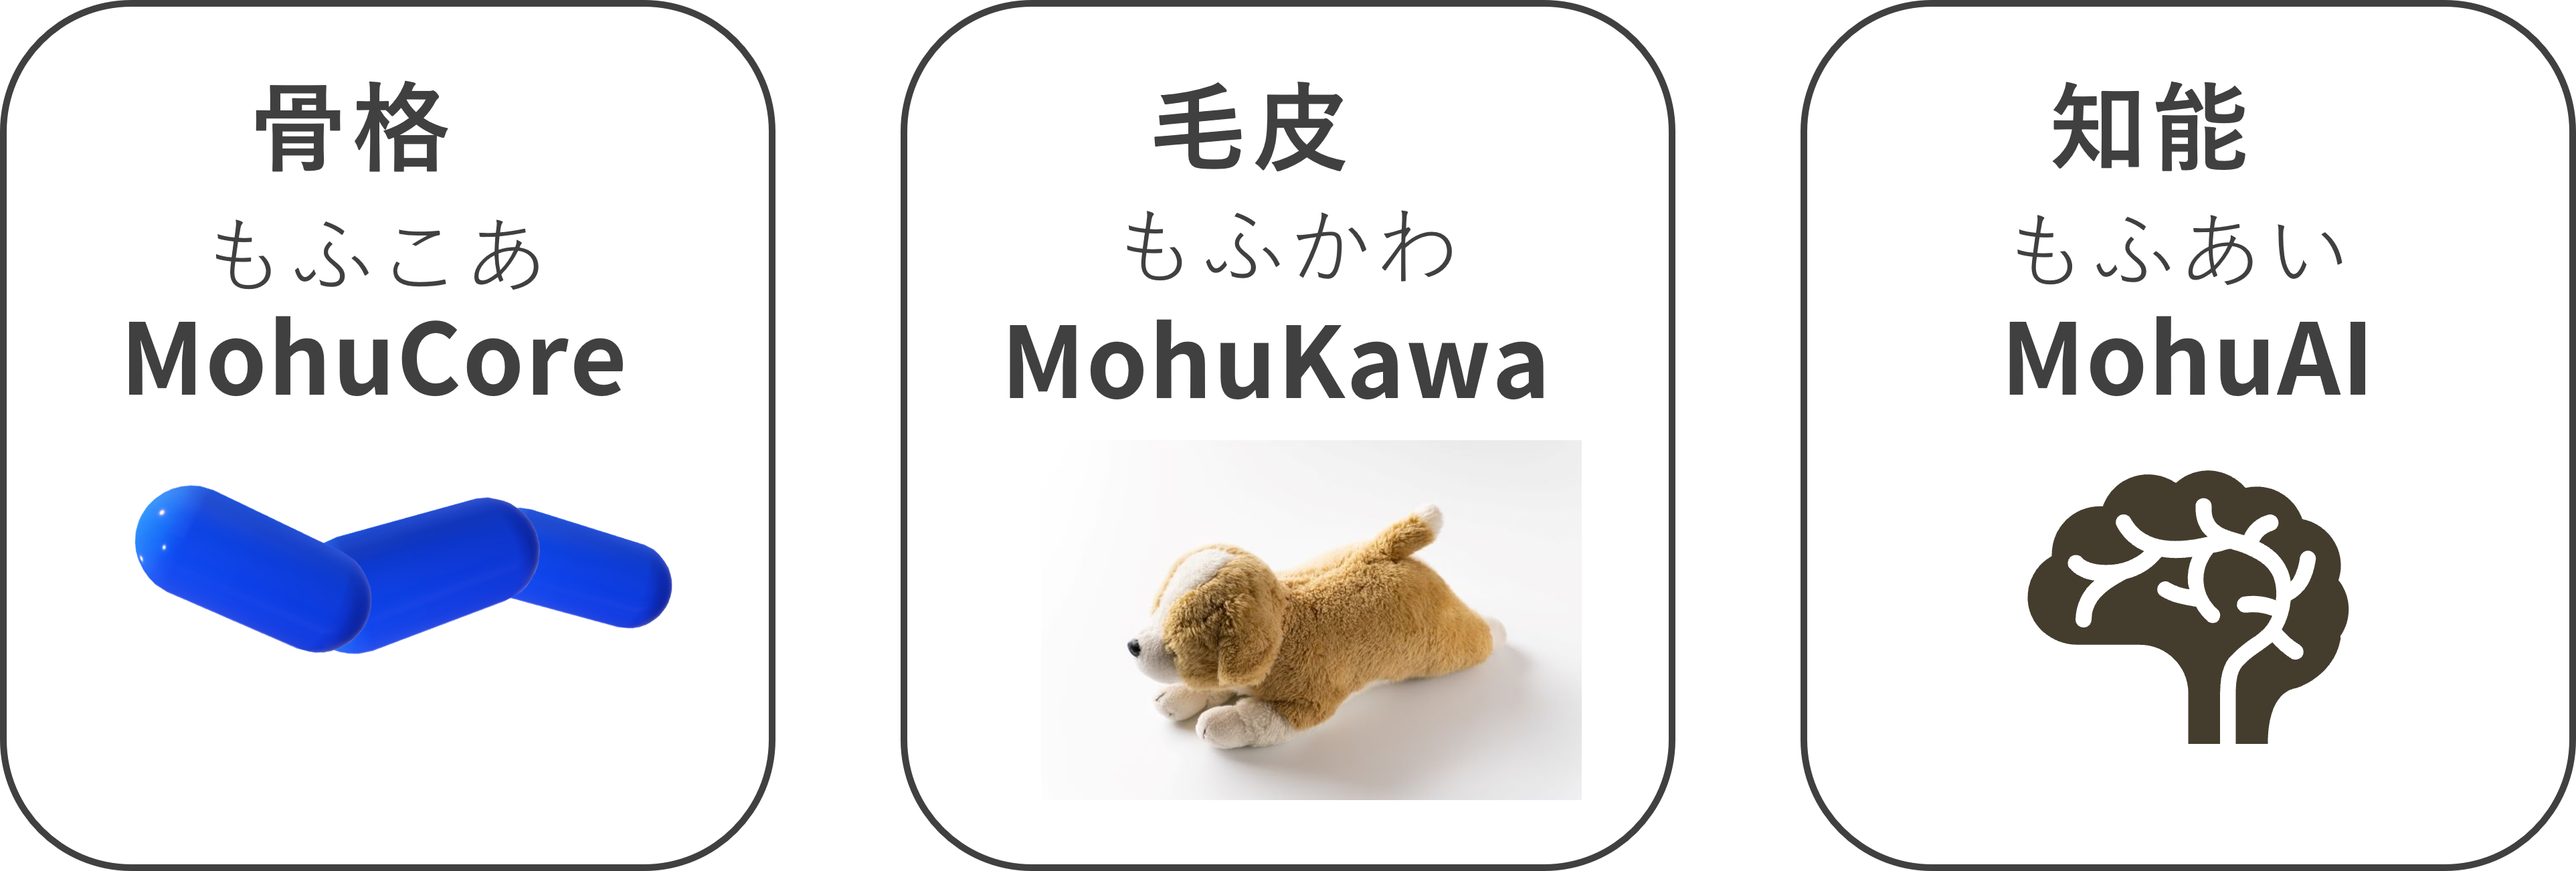
\includegraphics[width=12cm]{images/mohutics/concept.png}
  \caption{Mohuticsの構成}
  \label{fig:mohutics:concept}
\end{figure}

そして、開発の難所となるロボットのハードウェアやソフトウェアの共通化を進めることで、あらゆるぬいぐるみを効率的にロボット化することを目指した。

具体的には、まずはぬいぐるみロボットのセンサやアクチュエータ、制御基板等が含まれるロボットの骨格となるハードウェア部分MohuCoreを製作する。
ここで、MohuCoreは異なるぬいぐるみに接続可能な共通のハードウェアである点に注意する。

次に、ロボットの骨格MohuCoreを覆うようなぬいぐるみMohuKawaを製作する。
MohuKawaはぬいぐるみの外観に応じて犬やパンダなど、さまざまな種類が存在する。
しかし、これらにはすべて共通のジョイントが埋め込まれており、どの毛皮にも同じMohuCoreをその内部に組み込めるものとする。

さらに、ロボットに書き込むソフトウェアの総称をMohuAIとする。

そして、ユーザは共通の骨格MohuCoreと自分の好きなぬいぐるみの毛皮MohuKawaを用意し自ら組み合わせる(\figref{fig:mohutics:concept_embed})。
例えば、犬型のぬいぐるみに骨格を埋め込めば犬型のぬいぐるみロボットとなり(\figref{fig:mohutics:concept_dog})、熊型のぬいぐるみに同じ骨格を埋め込めば今度は熊型のぬいぐるみロボットとなる(\figref{fig:mohutics:concept_bear})。
最後に、ロボットのソフトウェアMohuAIを書き込むことで、自分の好きなぬいぐるみのロボットを簡単に手に入れることが可能となる。
\begin{figure}[htbp]
  \centering
  \begin{minipage}[c]{0.48\linewidth}
    \centering
    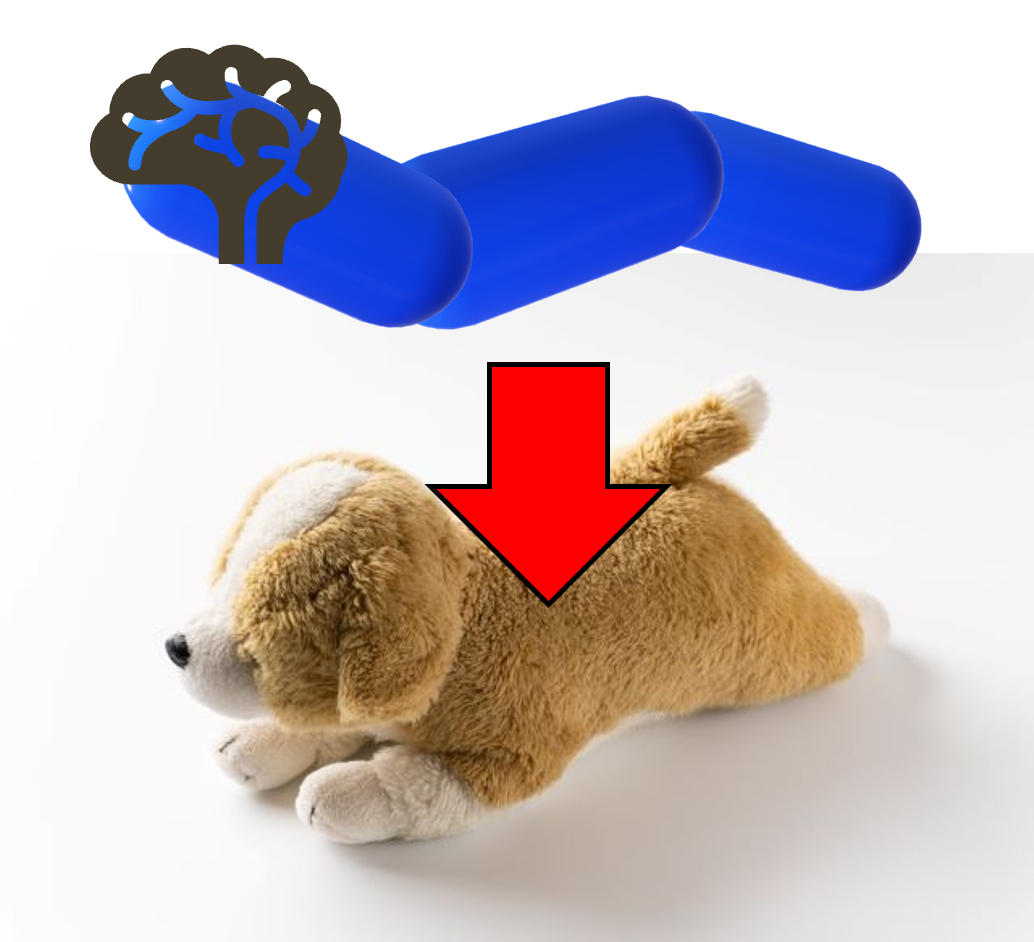
\includegraphics[keepaspectratio,width=4cm,clip]{images/mohutics/concept_dog.png}
    \subcaption{犬のぬいぐるみへの埋め込み}
    \label{fig:mohutics:concept_dog}
  \end{minipage}
  \begin{minipage}[c]{0.48\linewidth}
    \centering
    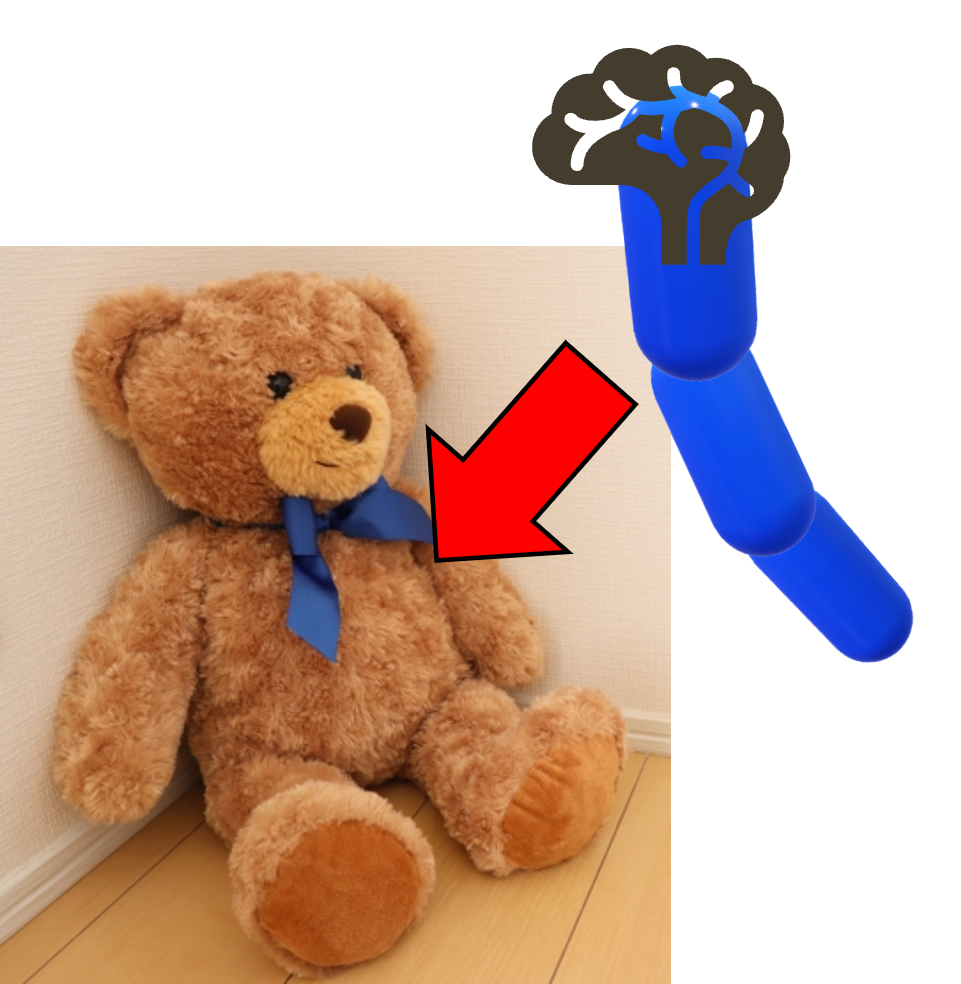
\includegraphics[keepaspectratio,width=4cm,clip]{images/mohutics/concept_bear.png}
    \subcaption{熊のぬいぐるみへの埋め込み}
    \label{fig:mohutics:concept_bear}
  \end{minipage}
  \caption{共通骨格を異なるぬいぐるみに埋め込む概念図}
  \label{fig:mohutics:concept_embed}
\end{figure}
以下では本プロジェクトで開発したMohuCore・MohuKawa・MohuAIそれぞれについて、その開発過程や機能をまとめる。

また、本プロジェクトで製作したぬいぐるみロボットMohuticsについて、複数のユーザに実際に触れ合ってもらい、聞き取りを行った。
その際のユーザからの評価についても記す。

\subsection{骨格MohuCoreの開発}
本プロジェクトのぬいぐるみロボットではぬいぐるみロボットの骨格を共通化することが求められる。
まずは動作を行うために必要なアクチュエータの種類と配置について検討を行った。

家電量販店等では犬型の電動で歩くおもちゃが販売されている(\figref{fig:dog_toy:body})。
このおもちゃを分解したところ、おもちゃ内部に樹脂製の骨格があり、一つのモータとギヤ、クラッチ等を使ってからくり人形のように機械仕掛けで動いていることがわかった(\figref{fig:dog_toy:skeleton})。
\begin{figure}[htbp]
  \centering
  \begin{minipage}[c]{0.48\linewidth}
    \centering
    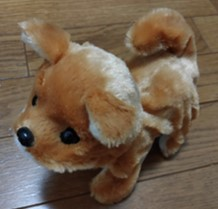
\includegraphics[keepaspectratio,width=4cm,clip]{images/dog_toy/dog.jpg}
    \subcaption{電動犬型おもちゃの外観}
    \label{fig:dog_toy:body}
  \end{minipage}
  \begin{minipage}[c]{0.48\linewidth}
    \centering
    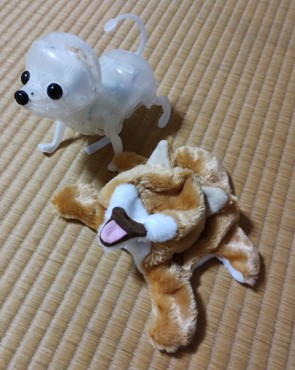
\includegraphics[keepaspectratio,width=4cm,clip]{images/dog_toy/skeleton.jpg}
    \subcaption{電動犬型おもちゃの内部骨格と毛皮}
    \label{fig:dog_toy:skeleton}
  \end{minipage}
  \label{fig:dog_toy}
\end{figure}

しかし、ギヤやクラッチを多用するとロボットとして間接を自由に動かすことは難しくなる。
そこで、本プロジェクトのMohuCoreではアクチュエータにサーボモータを使用することとした。

モータの配置について、例えばのような犬型やカンガルー型のものが考えられる。
これらの動物について、四肢に関節を埋め込んでぬいぐるみの脚を複雑に動かすことも可能であるが、骨格の構造を複雑にすればするほどぬいぐるみの形状に制約が生まれ、様々な種類のぬいぐるみに埋め込むことが難しくなってしまう。
よって、本プロジェクトではロボットを実際の動物の動きに近づけるのではなく、ぬいぐるみロボットとして必要十分な形状を目指し、最終的にMohuCoreはのような5関節のシリアルリンクロボットにした。
この構成では、例えば犬型ロボットの場合、頭が2自由度、腹の回転が1自由度、腰の回転が2自由度存在することになる。
本物の動物のように脚を自由に動かすことはできないが、ぬいぐるみロボットというコンセプトの下では十分に機能すると判断した。


\begin{figure}[htbp]
  \centering
  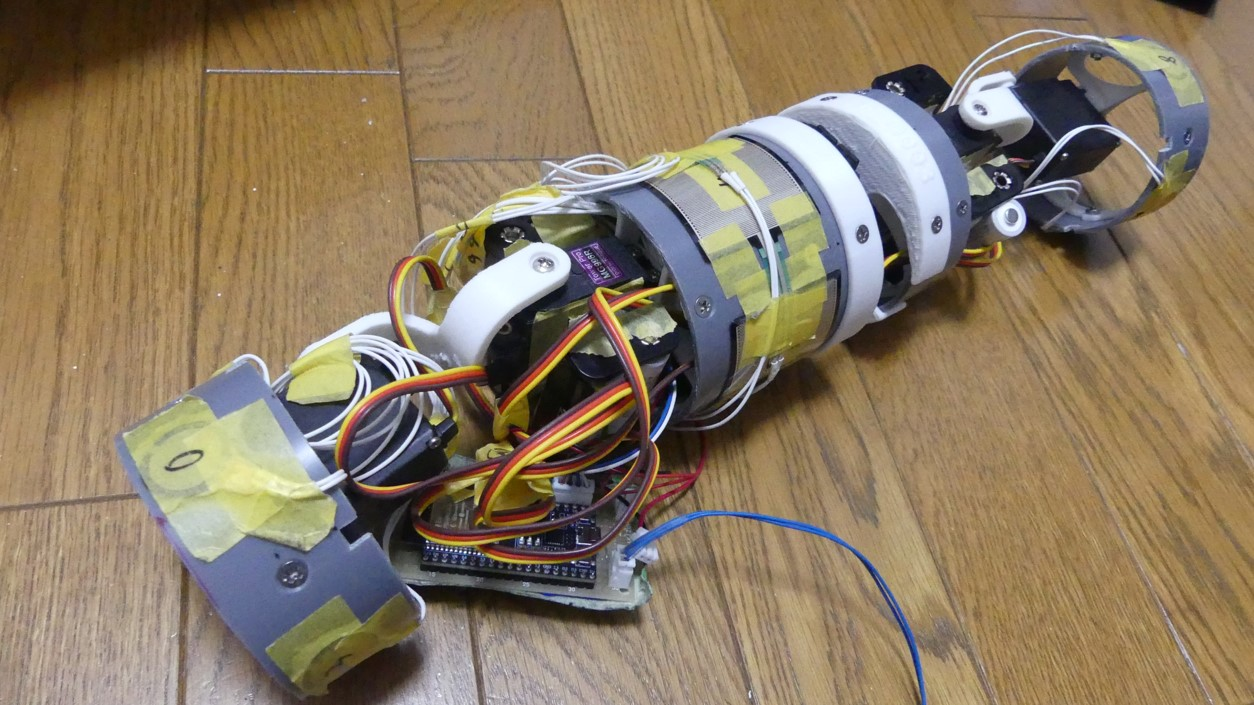
\includegraphics[width=8cm]{images/mohucore/skeleton.jpg}
  \caption{MohuCoreの外観}
  \label{fig::mohucore:skeleton}
\end{figure}

\subsection{毛皮MohuKawaの開発}

ロボットのぬいぐるみ部分となるMohuKawaについては、大きく分けて以下の二つの方法で製作した。
\begin{description}
  \item[ぬいぐるみを展開図から完全新規設計]犬型
  \item[市販のぬいぐるみをMohutics対応形状に改造]人型・アナゴ型・パンダ型  
\end{description}

ぬいぐるみを本プロジェクトのために完全新規設計したものとしては、犬型のぬいぐるみを用意した。
Mohuticsではぬいぐるみの内部に骨格となるMohuCoreを埋め込む必要があるため、ぬいぐるみ自体をMohuCoreに合わせて製作することが望ましい。
よって、犬型のぬいぐるみについては筆者が展開図の設計から縫製までをすべて行った。

一方で、世の中にはすでに数多くのぬいぐるみが存在するため、ユーザによってはすでに存在するぬいぐるみを使用したい場合があると想定される。
また、後述するとおり、ぬいぐるみの新規設計はやや難易度が高い。
そのため、ユーザの中には、手芸が得意で市販品の改造程度であれば問題なく行えるが新規設計するほどの時間や技術がないという者も一定数いると考えられる。
そこで、本プロジェクトでは新規設計のぬいぐるみだけでなく市販のぬいぐるみをMohuticsに対応するよう改造したものも製作した。
人型・アナゴ型・パンダ型のぬいぐるみは市販品の内部をくり貫くように加工している。

以下では、両者の方法について、その製作の過程や内容をまとめる。

\subsubsection{完全新規設計のMohuKawa}


\begin{figure}[htbp]
  \centering
  \begin{minipage}[c]{0.48\linewidth}
    \centering
    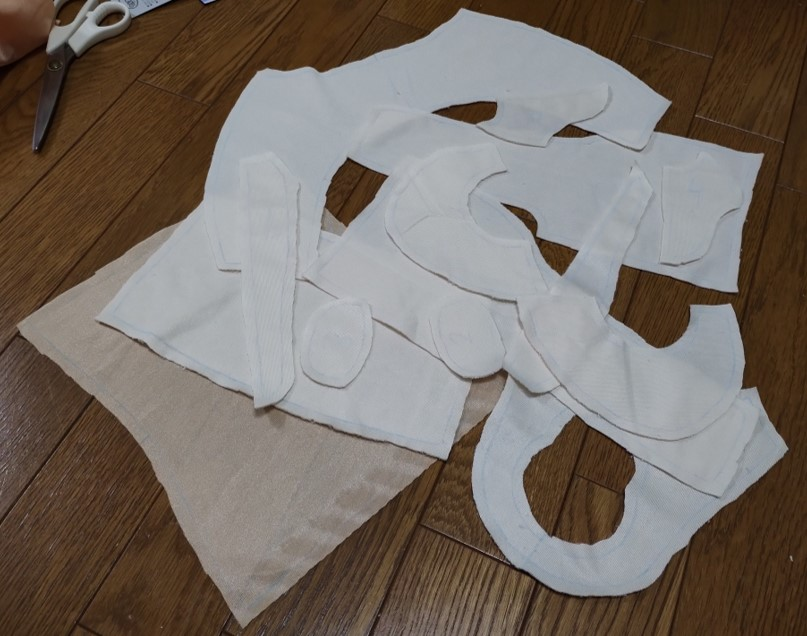
\includegraphics[keepaspectratio,width=4cm,clip]{images/mohukawa/saw_01.jpg}
    \subcaption{生地の裁断}
  \end{minipage}
  \begin{minipage}[c]{0.48\linewidth}
    \centering
    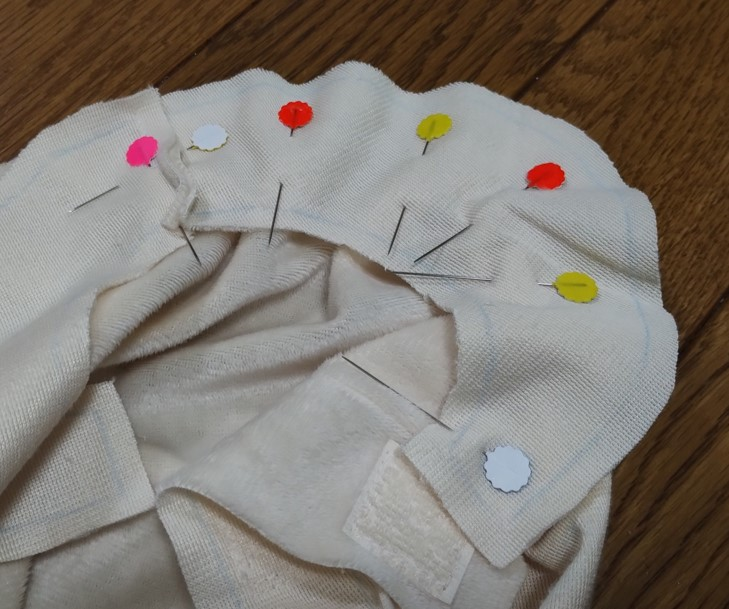
\includegraphics[keepaspectratio,width=4cm,clip]{images/mohukawa/saw_02.jpg}
    \subcaption{生地の縫製}
  \end{minipage} \\
  \begin{minipage}[c]{0.48\linewidth}
    \centering
    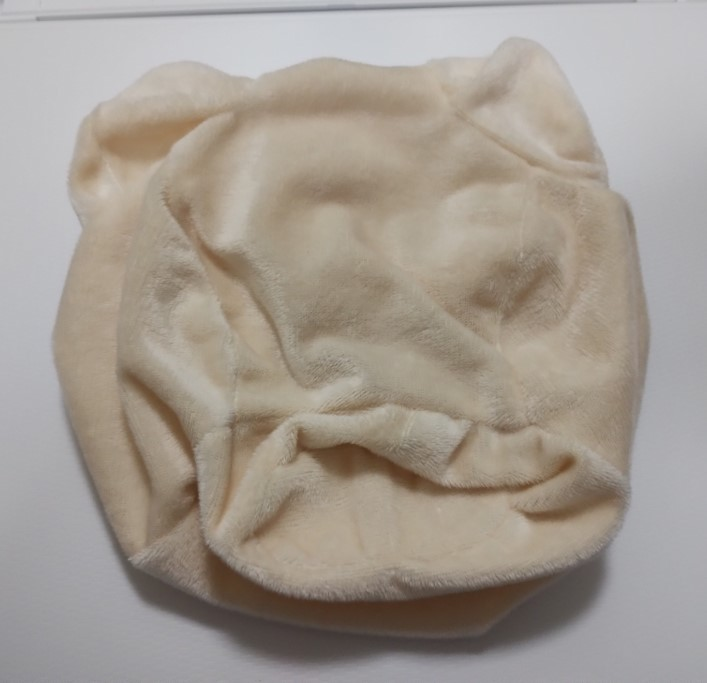
\includegraphics[keepaspectratio,width=4cm,clip]{images/mohukawa/saw_03.jpg}
    \subcaption{犬の頭部(前)}
  \end{minipage}
  \begin{minipage}[c]{0.48\linewidth}
    \centering
    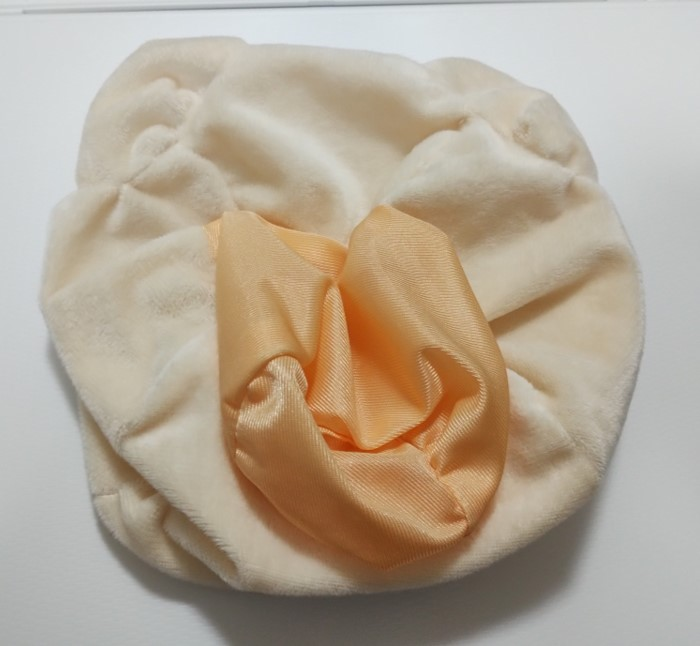
\includegraphics[keepaspectratio,width=4cm,clip]{images/mohukawa/saw_04.jpg}
    \subcaption{犬の頭部(前)}
  \end{minipage}
  \caption{犬のぬいぐるみの縫製の様子}
  \label{fig:mohukawa:saw}
\end{figure}

\begin{figure}[htbp]
  \centering
  \begin{minipage}[c]{0.48\linewidth}
    \centering
    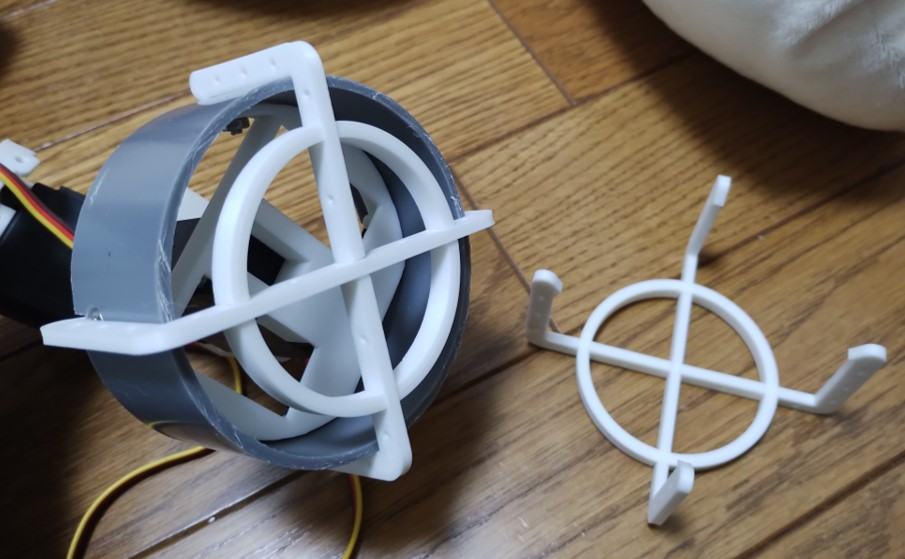
\includegraphics[keepaspectratio,width=4cm,clip]{images/mohukawa/joint_01.jpg}
    \subcaption{3Dプリンタで製作したジョイント}
  \end{minipage}
  \begin{minipage}[c]{0.48\linewidth}
    \centering
    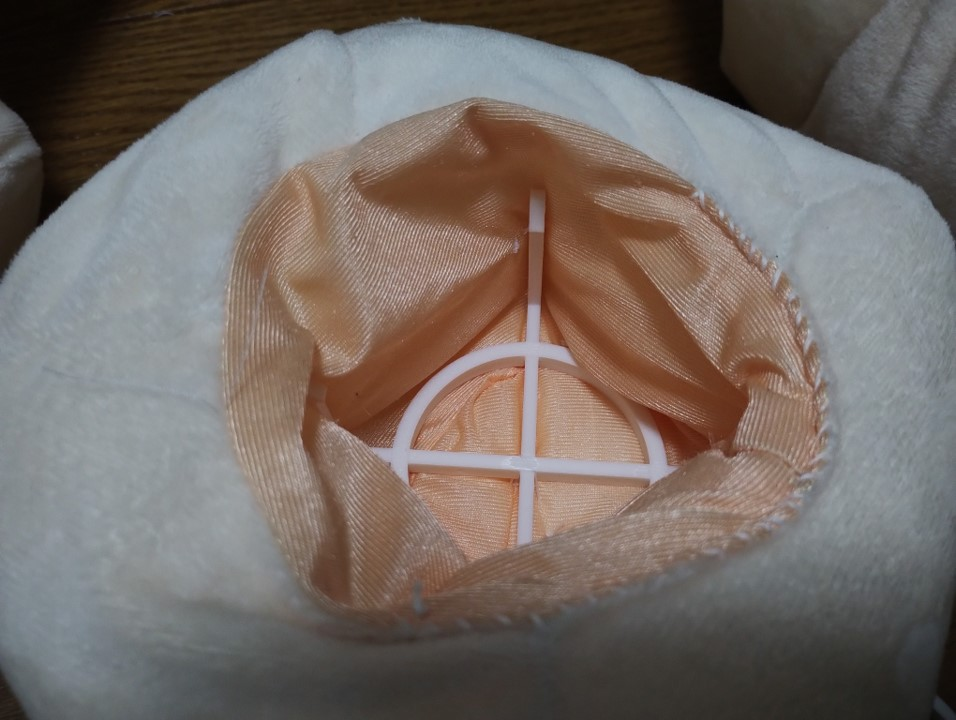
\includegraphics[keepaspectratio,width=4cm,clip]{images/mohukawa/joint_02.jpg}
    \subcaption{ジョイントの埋め込み}
  \end{minipage}
  \caption{犬のぬいぐるみへのジョイントの取り付け}
  \label{fig:mohukawa:joint}
\end{figure}


\subsubsection{市販品を改造して製作されたMohuKawa}


\subsection{知能MohuAIの開発}

ロボット開発では、ハードウェアとの入出力を直接扱う低レイヤー層やロボットの動作計画等のハードウェアを直接触れない高いレイヤーの層を異なるパッケージにまとめるなど、ハードウェア等への依存度に応じてプログラムを階層化させることが一般的である。
Mohuticsではロボットの電気的・機械的要素を含む骨格は共通化させるため、ぬいぐるみロボットの種類にかかわらず必要なハードウェア関連のソースコードは使いまわせる。
開発ではソースコードをぬいぐるみの種類や盛り込む機能に応じて共通化できる部分とそうでない部分に分割し、開発を進めた。

\subsection{ぬいぐるみロボットの完成}
\subsection{ユーザ評価}

\section{開発成果の特徴}

\section{今後の課題、展望}
本プロジェクトではシステムの簡素化及び省電力化を意図し、ロボットをESP32という比較的計算能力の低いマイクロコントローラを用いて設計した。
しかし、機械学習のスタンドアロンな実装やクラウドサービス等の連携を踏まえると、Linuxといった高機能なOSを搭載可能なシングルボードコンピュータを用いた方が発展性に富む。

本プロジェクト後半では、Raspberry Pi Zero 2Wという組み込み開発向けLinuxボードを使用し、計算能力を大幅に向上させた改良型も製作した(\figref{fig:prototype_04})。
この改良型では、サーボモータについても電流制御等が可能で動きも滑らかな高性能なものを搭載し、ぬいぐるみロボットとしての抱き心地を改善している。

\begin{figure}[htbp]
  \centering
  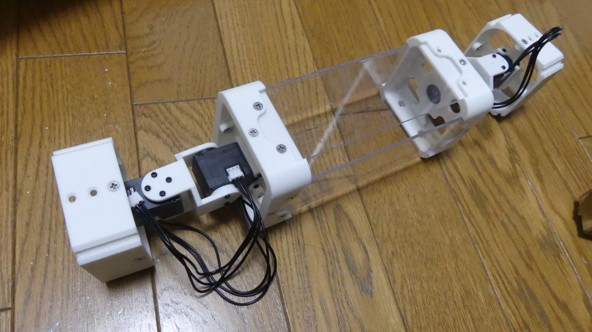
\includegraphics[width=8cm]{images/prototype/prototype_04.jpg}
  \caption{2024年3月現在開発中の改良型MohuCore}
  \label{fig:prototype_04}
\end{figure}

今後、ROS2といった汎用的なロボット開発フレームワークにプログラムコードを移植し、カメラや機械学習、クラウドなどとの連携が容易になる土台を整えてから、ぬいぐるみロボットのさらなる機能強化を進めたいと考えている。

展望としては、本プロジェクトで製作したぬいぐるみロボットシステムの開発を進め、いずれは製品として社会に広めることを目標としている。

まず、開発の大きな目標としては、本プロジェクトのロボットに人工知能分野の技術をさらに盛り込むことが考えられる。
現時点ではロボットが姿勢や触覚センサから機械学習を用いてユーザのロボットとの触れ合い方を認識し、それに応じた動作パターンを行う等の機能が実装されている。
これを発展させていけば、ロボットがユーザの表情やしぐさを読み取ってユーザが好む振る舞いを自ら学習したりできるであろう。

また、近年注目されるXR分野への適用も期待される。
インターネット上の仮想空間で会話を行えるVRChatのようなサービスに自身が抱いているぬいぐるみロボットを持ち込むことや、遠方の家族とぬいぐるみを通して握手や会話といったインタラクションを行うことは2024年3月現在開発中のハードウェアで実現可能だと考えている。

次に、本プロジェクトの社会への普及についても述べる。

ぬいぐるみロボットシステムMohuticsの特徴として、ぬいぐるみロボットに必要なロボットの開発とぬいぐるみの製造という全く異なる技術を、それぞれMohuCoreやMohuKawaなどとして適切に分割した点にある。
これにより、共通化されたロボット部分のMohuCoreはロボット開発が得意な筆者を中心とした組織が設計・開発し、多くの種類が必要でかつ縫製のノウハウも求められるMohuKawaはぬいぐるみメーカーに製造を委託するといったことが可能になる。
将来的にはMohuKawaを製造する各ぬいぐるみメーカーにMohutics対応を謳うためのライセンスを販売し、その収益をMohuCoreの開発に活用するといったビジネスモデルも考えられる。

さらに、ロボットのソフトウェア部分のMohuAIはオープンソースにすることが重要だと考えている。
本プロジェクトで開発したMohuticsは、ユーザの多様な好みに寄り添うためのぬいぐるみロボットを目指している。
しかし、ソフトウェアによってロボットに様々な機能が搭載できたとしても、それがユーザの需要を満たせるとは限らないし、ユーザが見つけても筆者が気づかなかったぬいぐるみロボットの新たな可能性を見落とすことになりかねない。
よって、ソースコードを公開し意欲のあるユーザにはプログラムを改変する余地を残すことが、ぬいぐるみロボットという発展途上の分野を育む上で重要だと考えている。

さらに、ぬいぐるみロボットは動物と異なり明確な死がないため、その運用は10年や20年といった長期に渡る可能性がある。
電子機器ではしばしば製造メーカーのソフトウェアの保守期間の終了が機器の運用に終わりを告げることがあるが、大手メーカーでもない限り、長期的なサポートをユーザに約束することは難しい。
特にぬいぐるみロボットは人の心に寄り添う愛玩対象であるため、メーカー側の都合でサポートが途切れることは避けることが望ましい。
したがって、ソフトウェアをオープンソースとし、Mohuticsが一定の技術を持つ有志の手で保守可能であると明示することが購買に関心のある客の安心感につながり、結果的にぬいぐるみロボットの長期的な発展につながると考えている。


\section{実施計画書内容との相違点}


% \section{開発分担}

\section{成長の自己分析}
本プロジェクトではロボットの設計及び製作、ぬいぐるみの設計及び製作、ソフトウェアの作成等を一貫して行った。
その中で、ロボットの製作で何度かスクラップビルドを繰り返すなど、ハードウェアとソフトウェアともに実装能力が向上した。

しかし、一番大きな成長は、プロジェクトを進めるにあたって、本当に必要な要素は何かを常に考え、取捨選択しつつ開発を進めた点にあると考える。
ぬいぐるみロボットとはユーザの感情に訴えかける製品であり、その評価軸は必ずしも明確ではない。
今まで電子工作の技能をもっぱら自身の趣味や純粋な性能のみが重視される大学内のプロジェクトなどに捧げてきた身としては、自分の作った物についてユーザの生の声を聞き、改良に活かす本プロジェクトは非常に新鮮であり貴重な機会であった。
そして、ユーザの指摘によって自分では気づかなかったぬいぐるみロボットの問題点や新たな魅力に気づき、人との対話が製品開発には必須だと改めて気づかされることとなった。

また、未踏IT人材発掘・育成事業を通して、さまざまなPMの方々や同期のクリエータと交流が行えたことも自身の成長につながっていると考えている。
これまで大学等でものづくりについて話題を共有できる相手がほとんどおらず、孤独を感じることが多かった。
本事業では意欲のある同期のクリエータと合宿や私的な交流を通して様々な話題について議論を行った。
その内容は、各々の本事業におけるプロジェクトについてだけでなく、本事業の枠を超えた技術的・社会的問題など多岐にわたる。
本事業には所属に関係なく多様な背景や関心を持つ人材が集まっており、本事業がなければ接することのなかったであろう人々と深く討論した時間は実に有意義なものとなった。

さらに、本プロジェクトの開発作業ではないものの、本プロジェクトと関連して、後述する商標出願等の手続きを自ら行った。
開発プロジェクトを長期的に進めるには、IT技術者としての開発能力だけでなく行政等との手続きも必要不可欠である。
未踏事業に採択されたことがきっかけとなって、開発プロジェクトを進めるための包括的な力が養われた。

今後も本事業を通して得られた学びやつながりを大切にし、自身のさらなる成長に活かしたいと考えている。


\section{秘匿ノウハウの指定}
本プロジェクトのソースコード等は2024年3月現在公開していない。
今後開発が進めば設計図やソースコードの公開も検討している。

\section{その他}
本プロジェクトと関連して、商標の出願を行った。
以下に出願番号を記す。
\begin{description}
  \item[Mohutics] 商願2023-060477
  \item[MohuCore] 商願2023-060484
  \item[MohuKawa] 商願2023-060485
  \item[MohuAI] 商願2023-060487
\end{description}

\section{付録}

\subsection{用語説明}
\subsubsection*{Mohutics (もふてぃくす) \label{term:mohutics}}
本プロジェクトで提案されたぬいぐるみロボットシステム及びそのシステムを採用したぬいぐるみロボットを指す。

\subsubsection*{MohuCore (もふこあ)\label{term:mohucore}}
本プロジェクトで提案されたぬいぐるみロボットシステムMohuticsにおいて、電気的・機械的要素を含むぬいぐるみロボットの骨格部分を指す。
\subsubsection*{MohuKawa (もふかわ)\label{term:mohukawa}}
本プロジェクトで提案されたぬいぐるみロボットシステムMohuticsにおいて、換装可能なぬいぐるみ部分を指す。
\subsubsection*{MohuAI (もふあい)\label{term:mohuai}}
本プロジェクトで提案されたぬいぐるみロボットシステムMohuticsにおいて、ぬいぐるみロボットに埋め込まれるソフトウェア部分を指す。

\subsubsection*{ESP32 \label{term:esp32}}
Espressif Systems社から発売されている32bitマイクロコントローラの製品群。
Wi-FiやBluetoothの搭載を特徴とし、特にESP32シリーズのマイクロコントローラを搭載したモジュールESP32-DevkitCはIoT開発を中心に広く用いられている。

\subsubsection*{IoT (Internet of Things) \label{term:iot}}
家電や車、電子機器等の様々なものがインターネットに接続され、相互に情報交換する仕組み。
本プロジェクトのぬいぐるみロボットがIoT端末として機能する場合、自宅に置いたぬいぐるみロボットをインターネット空間を経由して遠隔から操作することなどが想定される。

\subsubsection*{Linux \label{term:linux}}
コンピュータのOS(オペレーティングシステム)の一種。
オープンソースで開発されており、用途に合わせてUbuntuやDebian、Raspberry Pi OSといった様々な派生形(ディストリビューション)が存在する。


\subsubsection*{シングルボードコンピュータ \label{term:sbc}}
手のひら程度の大きさの1枚の基板にコンピュータとして必要なほぼすべての機能や要素を実装したもの。
Raspberry Pi等が知られている。

\subsubsection*{Raspberry Pi \label{term:raspi}}
Raspberry Pi財団によって開発されているARMプロセッサを搭載したシングルボードコンピュータ。
OSとしてLinuxベースのUbuntu等が使用可能な一方で、ハードウェア制御に便利な外部入出力端子を備えており、主にロボットやIoT等の組み込み用途の開発で用いられている。

\subsubsection*{ROS2 (Robot Operating System 2) \label{term:ros2}}
オープンソースのロボット用のソフトウェアプラットフォーム。
ロボットを構成するセンサやアクチュエータといった要素(ノード)同士のメッセージ通信やプログラムのパッケージ管理等を簡潔に行える。

\subsubsection*{XR}
Extended realityまたはCross realityと呼ばれる、現実世界と仮想世界を融合することで現実にないものを知覚できる技術の総称。
VR(仮想現実)やAR(拡張現実)、MR(複合現実)といった技術を含む。

\subsection{関連Webサイト}
\begin{description}
  \item[X: \url{https://twitter.com/mohutics}]\mbox{}\\
  プロジェクトの進捗をXのアカウントに随時掲載予定である。
  \item[GitHub: \url{https://github.com/mohutics}]\mbox{}\\
  今後ソースコードやロボットの設計図を公開する際は、このGitHubのアカウントに公開用リポジトリを掲載する予定である。
\end{description}





\bibliography{references}
\bibliographystyle{junsrt}

\end{document}
